\documentclass{beamer} %

%%%BASICS
\usepackage[utf8]{inputenc}
\usepackage{csquotes}
\usepackage{tikz}
\usepackage{verbatim}
\usepackage{amsmath}
\usepackage{amsfonts}
\usepackage{amsthm}
\usepackage{mathrsfs}
\usepackage{mathtools}

%%%START THEME SETTINGS
\usetheme{Dresden}
\usecolortheme{beaver}
\usefonttheme{professionalfonts}
%%%END THEME SETTINGS

%%%START APA
\usepackage[british]{babel}
\usepackage[backend=biber,style=apa]{biblatex}
\DeclareLanguageMapping{british}{british-apa}
%% APA citing
%% \cite{t} - Uthor und Richter, 2010
%% \textcite{t} - Uthor und Riter (2010)
%% \parencite{t} - (Uthor & Riter, 2010)
%% \parencite[Chapt.~4]{t} - (Uthor & Riter, 2010, S. 15)
%%%END APA

% Math Utils
\newcommand{\inner}[2]{\langle#1,\,#2\rangle}
\newcommand{\innerone}[1]{\langle#1\rangle}
\newcommand{\paren}[1]{\left(#1\right)}
\newcommand{\bracket}[1]{\left[#1\right]}
\newcommand{\given}{\biggr\rvert}
\newcommand{\PP}[1]{\mathbb{P}\paren{#1}}
\newcommand{\PPB}[1]{\mathbb{P}\bracket{#1}}
\newcommand{\PPP}{\mathbb{P}}
\newcommand{\E}{\mathbb{E}}
\newcommand{\EE}[1]{\mathbb{E}\paren{#1}}
\newcommand{\EEB}[1]{\mathbb{E}\bracket{#1}}
\newcommand{\Tr}[1]{\text{Tr}\paren{#1}}
\newcommand{\R}{\mathbb{R}}
\newcommand{\Z}{\mathbb{Z}}
\newcommand{\Q}{\mathbb{Q}}
\newcommand{\N}{\mathbb{N}}
\newcommand{\xeq}[1]{\stackrel{#1}{=}}
\newcommand{\indist}{\mathcal{D}}
\newcommand{\inprob}{\mathcal{P}}
\newcommand{\borel}{\mathcal{B}}
\newcommand{\indic}[1]{\mathbbm{1}_{#1}}
\newcommand\restr[2]{{% we make the whole thing an ordinary symbol
 \left.\kern-\nulldelimiterspace% automatically resize the bar with \right
 #1 % the function
 \vphantom{\big|} % pretend it's a little taller at normal size
 \right|_{#2} % this is the delimiter
}}
\newcommand{\im}{\text{Im}}
\newcommand{\cov}[2]{\text{Cov}\paren{#1,#2}}
\newcommand{\corr}[2]{\text{Corr}\paren{#1,#2}}
\newcommand{\var}[1]{\text{Var}\paren{#1}}
\newcommand{\abs}[1]{\left\lvert#1\right\rvert}
\newcommand{\norm}[1]{\vert\vert#1\rvert\rvert}
\newcommand{\grad}{\nabla}
\newcommand{\varrow}{\overset{\rightharpoonup}}
\newcommand{\diag}[1]{\text{diag}\paren{#1}}
\newcommand{\mesh}{\text{mesh}}
\newcommand{\sgn}[1]{\text{sgn}\paren{#1}}
\newcommand{\set}[1]{\{#1\}}
\newcommand{\swap}{\operatorname{swap}}

\newcommand{\code}[1]{{\texttt{\textcolor{mygray}{\small #1}}}}

\newcommand{\normal}[1]{\operatorname{\mathcal{N}}\paren{#1}}

\usepackage{amssymb}% http://ctan.org/pkg/amssymb
\usepackage{pifont}% http://ctan.org/pkg/pifont
\newcommand{\cmark}{\ding{51}}%
\newcommand{\xmark}{\ding{55}}%

% COLORS
\usepackage{color}
\usepackage{xcolor}
\definecolor{mygray}{rgb}{0.4,0.4,0.4}

\title{Overview of Automatic Differentiation}
\author{James Yang}
\date{\today}

\begin{document}

\begin{frame}
	\titlepage
\end{frame}

\begin{frame}
	\tableofcontents
\end{frame}

%------------------------------------------------------
\section{Introduction}

In a wide range of areas such as
optimization, statistical inference, quantitative finance, and physics,
the gradient, or total derivative, of a scalar function 
has proven to be essential when constructing algorithmic solutions to complex problems.
The simplest example in (convex) optimization is a root-finding algorithm such as Newton-Raphson method,
which updates a proposal value $x_n$ at every iteration by $-\frac{f(x_n)}{f'(x_n)}$.
In Bayesian statistics, there has been much development in advanced MCMC algorithms
such as the Hamiltonian Monte Carlo (HMC) and NUTS (No-U-Turn-Sampler),
which heavily rely on computing the gradient of 
a (log) joint probability density function~\cite{hoffman:2011}\cite{neal:2012}.
Modern neural networks also rely on computing 
the gradient of a loss function during back-propogation~\cite{goodfellow:2016}.


In quantitative finance, 

Often times, the target function to differentiate is quite complicated

\section{Forward-Mode Automatic Differentiation}
\frame{\tableofcontents[currentsection]}

\begin{frame}{Example Function and Expression Graph}
\[(x(t), y(t)) = (\cos(\omega t), \sin(\omega t))\]

\pause%
% Original expression graph
\begin{figure}[t]
\centering
\scalebox{0.9}{%

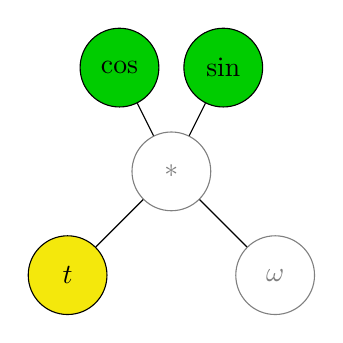
\begin{tikzpicture}[x=0.75pt,y=0.75pt,yscale=-0.5,xscale=0.5]

    \draw (200,350) node [align=center, minimum size=1cm, draw, circle, fill=black!5!yellow] (t)  {$t$};
    \draw (400,350) node [align=center, minimum size=1cm, draw, circle, color=gray] (omega)  {$\omega$};
    \draw (300,250) node [align=center, minimum size=1cm, draw, circle, color=gray] (mul) {$*$};
    \draw (250,150) node [align=center, minimum size=1cm, draw, circle, fill=black!20!green] (cos) {$\cos$};
    \draw (350,150) node [align=center, minimum size=1cm, draw, circle, fill=black!20!green] (sin) {$\sin$};
    \draw (t) -- (mul);
    \draw (omega) -- (mul);
    \draw (mul) -- (cos);
    \draw (mul) -- (sin);

\end{tikzpicture}
} % end scalebox

\end{figure}
\end{frame}

\begin{frame}{Forward AD}
\begin{itemize}
    \item Each node is represented by a \emph{dual number}, $(w, \frac{dw}{dx})$.
    \item Extend elementary functions to dual numbers.
    \item Unary $f$:
    \begin{align*}
        f( (w, \frac{dw}{dx}) ) := \paren{f(w), \frac{df}{dw} \frac{dw}{dx}}
    \end{align*}
    \item Binary $f$:
    {\small
    \begin{align*}
        f\paren{(w_1,\frac{dw_1}{dx}), (w_2, \frac{dw_2}{dx})}
        :=
        \paren{f(w_1,w_2), \frac{df}{dw_1} \frac{dw_1}{dx} + \frac{df}{dw_2}\frac{dw_1}{dx}}
    \end{align*}
    }
\end{itemize}
\end{frame}

\begin{frame}{Forward AD}
\begin{itemize}
    \item Example: 
    \begin{align*}
        \sin( (w, \frac{dw}{dx}) ) &= (\sin(w), \cos(w) \frac{dw}{dx})
        \\
        (w_1, \frac{dw_1}{dx}) \cdot (w_2, \frac{dw_2}{dx})
        &=
        (w_1 w_2, \frac{dw_1}{dx} w_2 + w_1 \frac{dw_2}{dx})
    \end{align*}
\end{itemize}    
\end{frame}

\begin{frame}{Forward AD Evaluation}
\begin{figure}[t]
\centering
\scalebox{0.9}{%

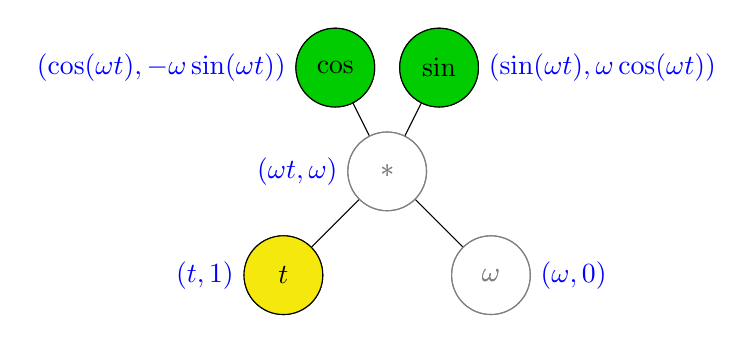
\begin{tikzpicture}[x=0.75pt,y=0.75pt,yscale=-0.5,xscale=0.5]

    \draw (200,350) node [align=center, minimum size=1cm, draw, circle, fill=black!5!yellow] (t)  {$t$};
    \draw (400,350) node [align=center, minimum size=1cm, draw, circle, color=gray] (omega)  {$\omega$};
    \draw (300,250) node [align=center, minimum size=1cm, draw, circle, color=gray] (mul) {$*$};
    \draw (250,150) node [align=center, minimum size=1cm, draw, circle, fill=black!20!green] (cos) {$\cos$};
    \draw (350,150) node [align=center, minimum size=1cm, draw, circle, fill=black!20!green] (sin) {$\sin$};
    \draw (t) -- (mul);
    \draw (omega) -- (mul);
    \draw (mul) -- (cos);
    \draw (mul) -- (sin);

    \pause%
    \draw (200,350) node [align=center, minimum size=1cm,
                          draw, circle, fill=black!5!yellow,
                          label={[blue]left:$(t,1)$}] (t) {$t$};
                          
    \pause%
    \draw (400,350) node [align=center, minimum size=1cm,
                          draw, circle, color=gray,
                          label={[blue]right:$(\omega,0)$}] (omega) {$\omega$};
                          
    \pause%
    \draw (300,250) node [align=center, minimum size=1cm,
                          draw, circle, color=gray,
                          label={[blue]left:$(\omega t, \omega)$}] (mul) {$*$};
                          
    \pause%
    \draw (250,150) node [align=center, minimum size=1cm,
                          draw, circle, fill=black!20!green,
                          label={[blue]left:$(\cos(\omega t), -\omega \sin(\omega t))$}] (cos) {$\cos$};
                          
    \pause%
    \draw (350,150) node [align=center, minimum size=1cm,
                          draw, circle, fill=black!20!green,
                          label={[blue]right:$(\sin(\omega t), \omega \cos(\omega t))$}] (sin) {$\sin$};

\end{tikzpicture}
} % end scalebox

\end{figure}
\end{frame}

\begin{frame}{Forward AD}
\begin{itemize}
    \item Easy to implement.
    \item Fast for $f:\R^n \to \R^m$ where $m \gg n$ ($O(n)$ sweeps of computation graph).
    \item Useful in physics applications when differentiating w.r.t. time.
    \item Example code (\href{https://github.com/JamesYang007/FastAD-Report/blob/master/slides/stanford-01272022/examples/src/fwd_ad.cpp}{\code{fwd\_ad}}).
\end{itemize}
\end{frame}

\section{Reverse-Mode Automatic Differentiation}
\frame{\tableofcontents[currentsection]}

\begin{frame}
\frametitle{Example Function and Expression Graph}
\[f(x_1, x_2, x_3) = \sin(x_1) + \cos(x_2) \cdot x_3 - \log(x_3)\]

\pause%

% Original expression graph
\begin{figure}[t]
\centering
\scalebox{0.9}{%

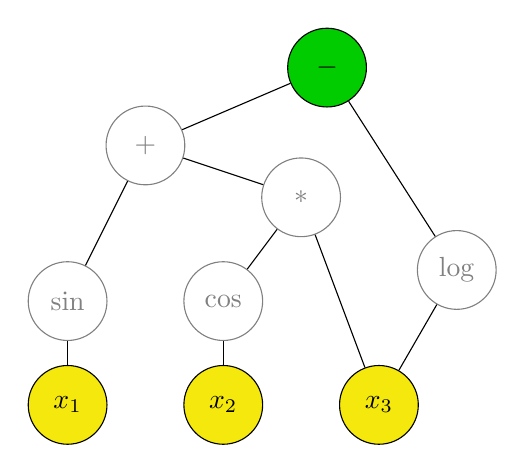
\begin{tikzpicture}[x=0.75pt,y=0.75pt,yscale=-0.5,xscale=0.5]

    \draw (150,350) node [align=center, minimum size=1cm, draw, circle, fill=black!5!yellow] (x1)  {$x_1$};
    \draw (300,350) node [align=center, minimum size=1cm, draw, circle, fill=black!5!yellow] (x2)  {$x_2$};
    \draw (450,350) node [align=center, minimum size=1cm, draw, circle, fill=black!5!yellow] (x3)  {$x_3$};
    \draw (150,250) node [align=center, minimum size=1cm, draw, circle, color=gray] (sin) {$\sin$};
    \draw (300,250) node [align=center, minimum size=1cm, draw, circle, color=gray] (cos) {$\cos$};
    \draw (525,220) node [align=center, minimum size=1cm, draw, circle, color=gray] (log) {$\log$};
    \draw (225,100) node [align=center, minimum size=1cm, draw, circle, color=gray] (add) {$+$};
    \draw (375,150) node [align=center, minimum size=1cm, draw, circle, color=gray] (mul) {$*$};
    \draw (400,25)  node [align=center, minimum size=1cm, draw, circle, fill=black!20!green] (sub) {$-$};
    \draw (x1) -- (sin);
    \draw (x2) -- (cos);
    \draw (x3) -- (mul);
    \draw (x3) -- (log);
    \draw (sin) -- (add);
    \draw (cos) -- (mul);
    \draw (mul) -- (add);
    \draw (add) -- (sub);
    \draw (log) -- (sub);

\end{tikzpicture}
} % end scalebox

\end{figure}
\end{frame}

% Explain what we modify to get from expr graph -> tree
\begin{frame}
\frametitle{Expression Tree Conversion}
\begin{itemize}
\item $x_i$ can be referenced by multiple nodes.
    \begin{itemize}
        \item e.g. $x_3$ is referenced by the \code{*} and \code{log} nodes.
    \end{itemize}

\item Convert expression graph into an expression tree.
    \begin{itemize}
        \item Replace all nodes with multiple parents as separate nodes
            that reference back to the actual variables.
    \end{itemize}

\item Mathematically,
\begin{align}
    f(x_1, x_2, x_3) &= \tilde{f}(g(x_1, x_2, x_3)) \label{eq:f-tree-example} \\
    \tilde{f}(w_1, w_2, w_3, w_4) &= \sin(w_1) + \cos(w_2) \cdot w_3 - \log(w_4) \nonumber \\
    g(x_1, x_2, x_3) &= (x_1, x_2, x_3, x_3) \nonumber
\end{align}

\end{itemize}
\end{frame}

% Expression tree
\begin{frame}
\frametitle{Expression Tree Conversion}

\begin{figure}[t]
\centering

\scalebox{0.9}{%

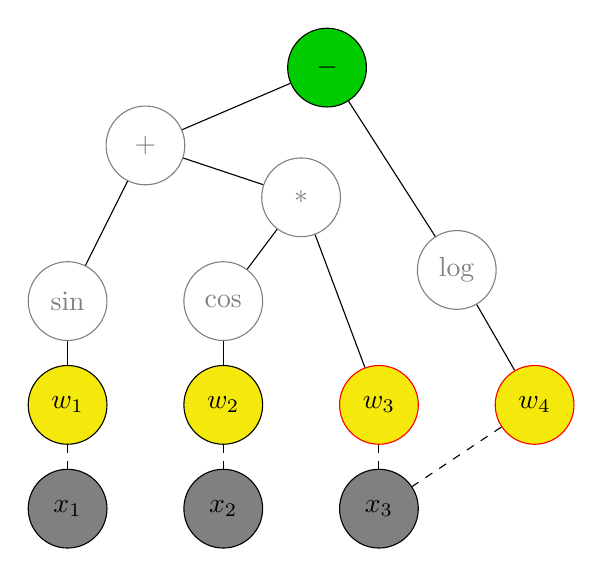
\begin{tikzpicture}[x=0.75pt,y=0.75pt,yscale=-0.5,xscale=0.5]

    \draw (150,450) node [align=center, minimum size=1cm, draw, circle, fill=gray] (x1)  {$x_1$};
    \draw (300,450) node [align=center, minimum size=1cm, draw, circle, fill=gray] (x2)  {$x_2$};
    \draw (450,450) node [align=center, minimum size=1cm, draw, circle, fill=gray] (x3)  {$x_3$};
    \draw (150,350) node [align=center, minimum size=1cm, draw, circle, fill=black!5!yellow] (w1)  {$w_1$};
    \draw (300,350) node [align=center, minimum size=1cm, draw, circle, fill=black!5!yellow] (w2)  {$w_2$};
    \draw (450,350) node [align=center, minimum size=1cm, draw=red, circle, fill=black!5!yellow] (w3)  {$w_3$};
    \draw (600,350) node [align=center, minimum size=1cm, draw=red, circle, fill=black!5!yellow] (w4)  {$w_4$};
    \draw (150,250) node [align=center, minimum size=1cm, draw, circle, color=gray] (sin) {$\sin$};
    \draw (300,250) node [align=center, minimum size=1cm, draw, circle, color=gray] (cos) {$\cos$};
    \draw (525,220) node [align=center, minimum size=1cm, draw, circle, color=gray] (log) {$\log$};
    \draw (225,100) node [align=center, minimum size=1cm, draw, circle, color=gray] (add) {$+$};
    \draw (375,150) node [align=center, minimum size=1cm, draw, circle, color=gray] (mul) {$*$};
    \draw (400,25)  node [align=center, minimum size=1cm, draw, circle, fill=black!20!green] (sub) {$-$};
    \draw [dashed] (w1) -- (x1);
    \draw [dashed] (w2) -- (x2);
    \draw [dashed] (w3) -- (x3);
    \draw [dashed] (w4) -- (x3);
    \draw (w1) -- (sin);
    \draw (w2) -- (cos);
    \draw (w3) -- (mul);
    \draw (w4) -- (log);
    \draw (sin) -- (add);
    \draw (cos) -- (mul);
    \draw (mul) -- (add);
    \draw (add) -- (sub);
    \draw (log) -- (sub);

\end{tikzpicture}

} % end scalebox

\end{figure}
\end{frame}

% Explain why we do conversion
\begin{frame}
\frametitle{Expression Tree Conversion}

\begin{itemize}

\item{Why do we need this conversion?}
    \begin{itemize}
        \item All nodes except \code{$x_i$} have exactly one parent.
        \item Leads to cleaner implementation.
        \item Better to treat $x_i$ as \emph{containers} for
            initial values and their \textbf{adjoints}, $\frac{\partial f}{\partial x_i}$,
            instead of nodes of the graph.
    \end{itemize}

\end{itemize}
\end{frame}

% Introduce AD algorithm
\begin{frame}
\frametitle{Reverse-Mode AD Algorithm}
\begin{itemize}

\item Assume for the moment that $f: \R^n \to \R$.

\item Reverse-mode algorithm consists of two passes of the expression tree:
    \begin{itemize}
        \item \emph{forward}-evaluation (not to be confused with forward-mode AD)
        \item \emph{backward}-evaluation
    \end{itemize}

\end{itemize}
\end{frame}

% Explain forward-evaluation
\begin{frame}
\frametitle{Forward-Evaluation}
\begin{itemize}

\item Compute expression in the usual fashion.
    \begin{itemize}
        \item Start at the root.
        \item Recursively forward-evaluate left to right all its children.
        \item Compute current node operation using children results.
            \begin{itemize}
                \item e.g.\ for \code{sin} node, $x_1 \to w_1 \to \sin(w_1)$
            \end{itemize}
    \end{itemize}

\end{itemize}
\end{frame}

% Continue explaining forward-eval with picture
\begin{frame}
\frametitle{Forward-Evaluation}
\begin{figure}[t]
\centering

\scalebox{0.9}{%

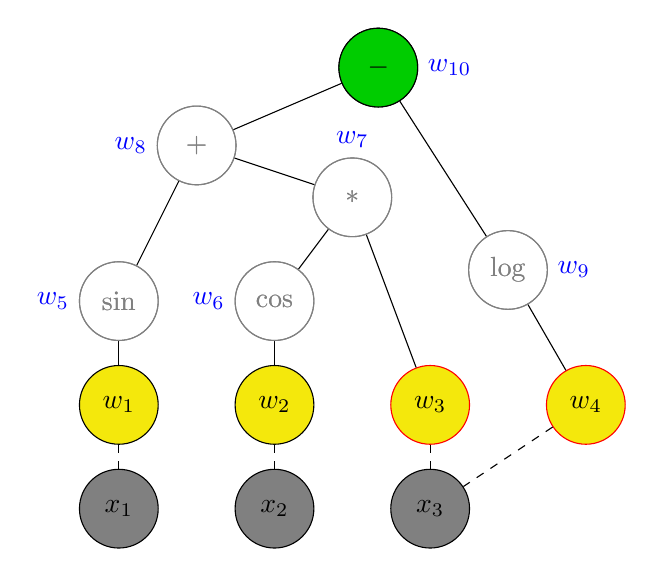
\begin{tikzpicture}[x=0.75pt,y=0.75pt,yscale=-0.5,xscale=0.5]

    \draw (150,450) node [align=center, minimum size=1cm, draw, circle, fill=gray] (x1)  {$x_1$};
    \draw (300,450) node [align=center, minimum size=1cm, draw, circle, fill=gray] (x2)  {$x_2$};
    \draw (450,450) node [align=center, minimum size=1cm, draw, circle, fill=gray] (x3)  {$x_3$};
    \draw (150,350) node [align=center, minimum size=1cm, draw, circle, fill=black!5!yellow] (w1)  {$w_1$};
    \draw (300,350) node [align=center, minimum size=1cm, draw, circle, fill=black!5!yellow] (w2)  {$w_2$};
    \draw (450,350) node [align=center, minimum size=1cm, draw=red, circle, fill=black!5!yellow] (w3)  {$w_3$};
    \draw (600,350) node [align=center, minimum size=1cm, draw=red, circle, fill=black!5!yellow] (w4)  {$w_4$};
    \draw (150,250) node [align=center, minimum size=1cm, draw, circle, color=gray] (sin) {$\sin$};
    \draw (300,250) node [align=center, minimum size=1cm, draw, circle, color=gray] (cos) {$\cos$};
    \draw (525,220) node [align=center, minimum size=1cm, draw, circle, color=gray] (log) {$\log$};
    \draw (225,100) node [align=center, minimum size=1cm, draw, circle, color=gray] (add) {$+$};
    \draw (375,150) node [align=center, minimum size=1cm, draw, circle, color=gray] (mul) {$*$};
    \draw (400,25)  node [align=center, minimum size=1cm, draw, circle, fill=black!20!green] (sub) {$-$};
    \draw [dashed] (w1) -- (x1);
    \draw [dashed] (w2) -- (x2);
    \draw [dashed] (w3) -- (x3);
    \draw [dashed] (w4) -- (x3);
    \draw (w1) -- (sin);
    \draw (w2) -- (cos);
    \draw (w3) -- (mul);
    \draw (w4) -- (log);
    \draw (sin) -- (add);
    \draw (cos) -- (mul);
    \draw (mul) -- (add);
    \draw (add) -- (sub);
    \draw (log) -- (sub);

    \pause%
    \draw (150,250) node [align=center, minimum size=1cm,
                          draw, circle, color=gray,
                          label={[blue]left:$w_5$}] (sin) {$\sin$};
    \pause%
    \draw (300,250) node [align=center, minimum size=1cm,
                          draw, circle, color=gray,
                          label={[blue]left:$w_6$}] (cos) {$\cos$};
    \pause%
    \draw (375,150) node [align=center, minimum size=1cm,
                          draw, circle, color=gray,
                          label={[blue]90:$w_7$}] (mul) {$*$};

    \pause%
    \draw (225,100) node [align=center, minimum size=1cm,
                          draw, circle, color=gray,
                          label={[blue]left:$w_8$}] (add) {$+$};

    \pause%
    \draw (525,220) node [align=center, minimum size=1cm,
                          draw, circle, color=gray,
                          label={[blue]right:$w_9$}] (log) {$\log$};
    \pause%
    \draw (400,25)  node [align=center, minimum size=1cm,
                          draw, circle, fill=black!20!green,
                          label={[blue]right:$w_{10}$}] (sub) {$-$};

\end{tikzpicture}

} % end scalebox

\end{figure}
\end{frame}

% Explain back-eval algorithm
\begin{frame}
\frametitle{Backward-Evaluation}
\begin{itemize}

\item Current node receives its adjoint from its parent.

\item This adjoint is also referred to as \emph{seed}.

\item Hence, root will receive seed = 1 from the caller.

\item Current node computes seeds for all its children and
    recursively backward-evaluates from \emph{right-to-left}.

\end{itemize}
\end{frame}

% Explain how to compute next seeds
\begin{frame}
\frametitle{Backward-Evaluation: Computing Next Seed}
\begin{itemize}

\item Next seed is computed by a simple chain-rule.
\item Let the current node be $w \in \R^{p \times q}$ and $v \in \R^{m \times n}$ one of its children.
\item The seed for $v$ is given by
\begin{align}
    \frac{\partial f}{\partial v_{ij}} &=
        \sum\limits_{k=1}^p \sum\limits_{l=1}^q
        \frac{\partial f}{\partial w_{kl}} \frac{\partial w_{kl}}{\partial v_{ij}}
    \label{eq:next-adj}
\end{align}
\item Since we are working with an expression tree,
    $f$ only depends on $v$ through $w$, hence this is the full adjoint.

\end{itemize}
\end{frame}

\begin{frame}
\frametitle{Backward-Evaluation: Computing Next Seed}
\begin{itemize}

\item Nodes with reference to containers must increment
    the adjoints in the containers with their seed.
    \begin{itemize}
        \item e.g.\ $w_3$ and $w_4$ increments the adjoint in $x_3$ with their seeds.
    \end{itemize}

\item Why? Chain-rule, once again.

\item Let $w_1, \ldots, w_k$ denote all variables with a reference to $x$.
    For simplicity assume they are all scalars (easily generalizable).
    Then,
    \begin{align*}
        \frac{\partial f}{\partial x}
        &=  \sum\limits_{i=1}^k
            \frac{\partial f}{\partial w_{i}} \frac{\partial w_{i}}{\partial x}
        =   \sum\limits_{i=1}^k
            \frac{\partial f}{\partial w_{i}}
    \end{align*}

\item Accumulated adjoints for $x_1, x_2, x_3$ is the gradient of $f$.

\end{itemize}
\end{frame}

% Back-eval with picture
\begin{frame}
\frametitle{Backward-Evaluation}
\begin{figure}[t]
\centering

\scalebox{0.9}{%

\begin{tikzpicture}[x=0.75pt,y=0.75pt,yscale=-0.5,xscale=0.5]

    \draw (150,450) node [align=center, minimum size=1cm, draw, circle, fill=gray] (x1)  {$x_1$};
    \draw (300,450) node [align=center, minimum size=1cm, draw, circle, fill=gray] (x2)  {$x_2$};
    \draw (450,450) node [align=center, minimum size=1cm, draw, circle, fill=gray] (x3)  {$x_3$};
    \draw (150,350) node [align=center, minimum size=1cm, draw, circle, fill=black!5!yellow] (w1)  {$w_1$};
    \draw (300,350) node [align=center, minimum size=1cm, draw, circle, fill=black!5!yellow] (w2)  {$w_2$};
    \draw (450,350) node [align=center, minimum size=1cm, draw=red, circle, fill=black!5!yellow] (w3)  {$w_3$};
    \draw (600,350) node [align=center, minimum size=1cm, draw=red, circle, fill=black!5!yellow] (w4)  {$w_4$};
    \draw (150,250) node [align=center, minimum size=1cm, draw, circle, color=gray] (sin) {$\sin$};
    \draw (300,250) node [align=center, minimum size=1cm, draw, circle, color=gray] (cos) {$\cos$};
    \draw (525,220) node [align=center, minimum size=1cm, draw, circle, color=gray] (log) {$\log$};
    \draw (225,100) node [align=center, minimum size=1cm, draw, circle, color=gray] (add) {$+$};
    \draw (375,150) node [align=center, minimum size=1cm, draw, circle, color=gray] (mul) {$*$};
    \draw (400,25)  node [align=center, minimum size=1cm, draw, circle, fill=black!20!green] (sub) {$-$};
    \draw [dashed] (w1) -- (x1);
    \draw [dashed] (w2) -- (x2);
    \draw [dashed] (w3) -- (x3);
    \draw [dashed] (w4) -- (x3);
    \draw (w1) -- (sin);
    \draw (w2) -- (cos);
    \draw (w3) -- (mul);
    \draw (w4) -- (log);
    \draw (sin) -- (add);
    \draw (cos) -- (mul);
    \draw (mul) -- (add);
    \draw (add) -- (sub);
    \draw (log) -- (sub);

    % Leftover labelling from forward-evaluation
    \draw (150,250) node [align=center, minimum size=1cm,
                          draw, circle, color=gray,
                          label={[blue]left:$w_5$}] (sin) {$\sin$};
    \draw (300,250) node [align=center, minimum size=1cm,
                          draw, circle, color=gray,
                          label={[blue]left:$w_6$}] (cos) {$\cos$};
    \draw (375,150) node [align=center, minimum size=1cm,
                          draw, circle, color=gray,
                          label={[blue]90:$w_7$}] (mul) {$*$};
    \draw (225,100) node [align=center, minimum size=1cm,
                          draw, circle, color=gray,
                          label={[blue]left:$w_8$}] (add) {$+$};
    \draw (525,220) node [align=center, minimum size=1cm,
                          draw, circle, color=gray,
                          label={[blue]right:$w_9$}] (log) {$\log$};
    \draw (400,25)  node [align=center, minimum size=1cm,
                          draw, circle, fill=black!20!green,
                          label={[blue]right:$w_{10}$}] (sub) {$-$};

    \pause%
    \draw [red] (sub) -- (log) node[midway, label={[red]right:$-1$}];

    \pause%
    \draw [red] (log) -- (w4) node[midway, label={[red]right:$\frac{-1}{w_4}$}];

    \pause%
    \draw [red, dashed] (w4) -- (x3) node[midway, label={[red]280:$\frac{-1}{w_4}$}];

    \pause%
    \draw [red] (sub) -- (add) node[midway, label={[red]100:$1$}];

    \pause%
    \draw [red] (add) -- (mul) node[midway, label={[red]90:$1$}];

    \pause%
    \draw [red] (mul) -- (w3) node[midway, label={[red]-20:$w_6$}];

    \pause%
    \draw [red, dashed] (w3) -- (x3) node[midway, label={[red]left:$w_6$}];

    \pause%
    \draw [red] (mul) -- (cos) node[midway, label={[red]100:$w_3$}];

    \pause%
    \draw [red] (cos) -- (w2) node[midway, label={[red]left:\scriptsize $-w_3\sin(w_2)$}];

    \pause%
    \draw [red, dashed] (w2) -- (x2) node[midway, label={[red]left:\scriptsize $-w_3\sin(w_2)$}];

    \pause%
    \draw [red] (add) -- (sin) node[midway, label={[red]100:$1$}];

    \pause%
    \draw [red] (sin) -- (w1) node[midway, label={[red]left:\scriptsize $\cos(w_1)$}];

    \pause%
    \draw [red, dashed] (w1) -- (x1) node[midway, label={[red]left:\scriptsize $\cos(w_1)$}];

\end{tikzpicture}

} % end scalebox
\end{figure}
\end{frame}

\begin{frame}{Backward-Evaluation}
\begin{itemize}
    \item Sanity check:
    \begin{align*}
        f(x_1, x_2, x_3) &= \sin(x_1) + \cos(x_2) \cdot x_3 - \log(x_3) \\
        \nabla f &= \paren{\cos(x_1), -x_3\sin(x_2), \cos(x_2)-x_3^{-1}}
    \end{align*}
\end{itemize} 
\end{frame}

\begin{frame}{Remarks}
\begin{itemize}
    \item Much harder to implement (memory management is tricky).
    \item Fast for $f:\R^n \to \R^m$ where $n \gg m$ ($O(m)$ sweeps of computation graph).
    \item Useful when we need to compute gradient (of a scalar function).
    \item Example code:
    \begin{itemize}
        \item \code{rv\_ad}
        \item \code{for\_each}
        \item \code{if\_else}
    \end{itemize}
\end{itemize} 
\end{frame}
\section{Tips}
\frame{\tableofcontents[currentsection]}

\begin{frame}{Reverse-Mode}
\begin{itemize}
    \item Extract common sub-expression into a placeholder variable, 
    to avoid recomputation, e.g.
    \begin{align*}
        t &= x + y \\
        f(t) &= \sin(t) \cos(t) 
    \end{align*}
    \item Use package-provided functions mostly to take advantage of vectorization, e.g.
    \begin{align*}
        \text{for-loop sum over } x \, &\text{ \xmark} \\
        \text{sum}(x) \, &\text{ \cmark} 
    \end{align*}
\end{itemize}
\end{frame}

\begin{frame}{Reverse-Mode}
\begin{itemize}
    \item Minimize number of nodes in computation graph,
    e.g. if $x \in \R^{10}$,
    \begin{align*}
        x[1] + \ldots + x[10] \implies 9 \, \text{ adjoints} \; &\text{ \xmark} \\
        \text{sum}(x) \; \implies 1 \, \text{ adjoint} \; &\text{ \cmark}
    \end{align*}
    \item Minimize size of each node of computation graph,
    e.g. if $x, y \in \R^n$,
    \begin{align*}
        \text{sum}(x+y) \implies O(n) \, \text{memory} \; &\text{ \xmark} \\
        \text{sum}(x) + \text{sum}(y) \implies O(1) \, \text{memory} \; &\text{ \cmark}
    \end{align*}
\end{itemize}
\end{frame}
\section{Applications}
\frame{\tableofcontents[currentsection]}

\begin{frame}{Taste of using AD}
\begin{itemize}
    \item MLE: Gaussian model.
    \item MLE: Gaussian mixture model.
    \item MAP: Ridge.
\end{itemize}
\end{frame}

\begin{frame}{MLE: Gaussian model}
\begin{itemize}
    \item $X_i \stackrel{iid}{\sim} N(\mu, 1)$ 
    \item $\mu$ unknown.
    \item Negative log-pdf is given by
    \begin{align*}
        -\sum\limits_{i=1}^n \log(p(x_i))
        =
        \frac{1}{2} \sum\limits_{i=1}^n (X_i - \mu)^2
    \end{align*}
    \item Example code (\href{https://github.com/JamesYang007/FastAD-Report/blob/master/slides/stanford-01272022/examples/src/mle.cpp}{\code{mle}}).
\end{itemize}
\end{frame}

\begin{frame}{MLE: Gaussian mixture model}
\begin{itemize}
    \item<2-> This is for you Kevin Senpai.
    \item<3-> $X_i \stackrel{iid}{\sim} \pi N(\mu_1, \sigma_1^2) + (1-\pi) N(\mu_2, \sigma_2^2)$ 
    \item<3-> $(\pi, \mu_1, \mu_2, \sigma_1, \sigma_2)$ unknown.
    \item<3-> Negative log-pdf is given by
    \begin{align*}
        -\sum\limits_{i=1}^n \log(p(x_i))
        =
        -\sum\limits_{i=1}^n \log\paren{
            \pi p_{\mu_1, \sigma_1}(X_i)
            + (1-\pi) p_{\mu_2, \sigma_2}(X_i)
        }
    \end{align*}
    \item<3-> Example code (\href{https://github.com/JamesYang007/FastAD-Report/blob/master/slides/stanford-01272022/examples/src/kevin_senpai_mle.cpp}{\code{kevin\_senpai\_mle}}).
\end{itemize}
\end{frame}

\begin{frame}{MAP: Ridge}
\begin{itemize}
    \item MLE is really just MAP of likelihood + non-informative prior.
    \item In general, can apply any (differentiable) prior.
    \item Ridge regression (fixed $X$): 
    \begin{align*}
        y | \beta &\sim \normal{X\beta, I} \\
        \beta &\sim \normal{0, \lambda^{-1}}
    \end{align*}
    \item MAP is posterior mean:
    \begin{align*}
        \EE{\beta | y}
        &=
        (X^\top X + \lambda I)^{-1} X^\top y
    \end{align*}
    \item Example code (\href{https://github.com/JamesYang007/FastAD-Report/blob/master/slides/stanford-01272022/examples/src/map.cpp}{\code{map}}).
\end{itemize} 
\end{frame}

\section{Benchmarks}
\frame{\tableofcontents[currentsection]}

\begin{frame}{Comparison with Finite Difference and Manual}
\begin{itemize}
    \item Example function: 
    $x \in \R^p$, $M \in \R^{n\times p}$
    \begin{align*}
        f(x) = \text{sum}(Mx) - 2\log(\sum\limits_{i=1}^p \exp{(x_i)})
    \end{align*}
    \item Code (\href{https://github.com/JamesYang007/FastAD-Report/blob/master/slides/stanford-01272022/examples/src/compare_fd.cpp}{\code{compare\_fd}})
\end{itemize} 
\begin{table}[t]
    \centering
    \resizebox{\linewidth}{!}{%
    \begin{tabular}{|c||c|c|c|c|}
        \hline
        Config & FD & AD & Manual (df only) & Manual (f + df) \\ \hline
        n=10, p=100 & 2.2e-3 & 5.78e-5 & 3.66e-5 & 4.31e-5 \\ \hline 
        n=10, p=10000 & NA & 4.3e-3 & 3.4e-3 & 4.1e-3 \\ \hline 
        n=100, p=10 & 1.1e-4 & 4.2-5 & 9.09e-6 & 1.61e-5 \\ \hline
        n=10000, p=10 & 8.56e-3 & 2.64e-3 & 3e-4 & 1e-3 \\ \hline
    \end{tabular}
    }
\end{table}
\end{frame}


\end{document}
